\documentclass[tikz,border=4pt]{standalone}
\usepackage{ctex}
\usepackage{amsmath}
\usetikzlibrary{calc, angles, quotes, arrows.meta}

\begin{document}
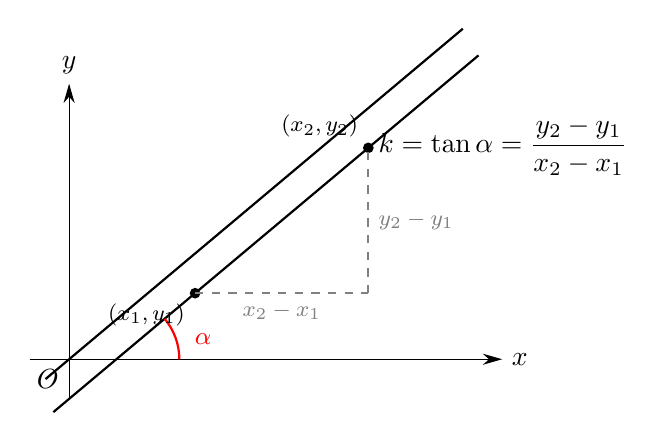
\begin{tikzpicture}[
  scale=1.0, thick,
  axis/.style={-{Stealth[length=7pt, width=4pt]}, thin},
  line/.style={{Stealth[length=6pt, width=3.5pt]}-{Stealth[length=6pt, width=3.5pt]}, thick},
]

% 坐标轴
\draw[axis] (-0.5,0) -- (5.5,0) node[right] {$x$};
\draw[axis] (0,-0.5) -- (0,3.5) node[above] {$y$};
\node[below left] at (0,0) {$O$};

% 直线 (穿越 x 轴正方向，倾斜角约 40°)
% 过原点附近，方向角 40°
\coordinate (P1) at (-0.3, -0.252);
\coordinate (P2) at (5.0, 4.197);

\draw[thick, black] (P1) -- (P2);

% 倾斜角弧
% 直线与 x 轴的交点
\coordinate (Q) at (0.6, 0);  % 交点近似

% 用更精确的交点：直线 y = tan(40°)*(x - 0.6) 过 (0.6,0)，tan40≈0.839
% 重新定义：直线过 (0.6, 0)，斜率 tan(40°)≈0.839
\coordinate (Q) at (0.6, 0);
\coordinate (LineStart) at (-0.2, {-0.839*0.8});
\coordinate (LineEnd) at (5.2, {0.839*(5.2-0.6)});

\draw[thick, black] (LineStart) -- (LineEnd);

% x 轴正方向辅助点（弧的终点方向）
\coordinate (Xpos) at (2.0, 0);

% 角弧：从 x 轴正方向到直线方向
\draw[red, thick] (Q) ++(0.8,0) arc[start angle=0, end angle=40, radius=0.8];

% 标注倾斜角 α
\node[red] at ($(Q) + (1.1, 0.25)$) {\small $\alpha$};

% 直线上取两点标注斜率
\coordinate (A) at (1.6, {0.839*(1.6-0.6)});
\coordinate (B) at (3.8, {0.839*(3.8-0.6)});

\filldraw[black] (A) circle (1.5pt) node[below left] {\footnotesize $(x_1,y_1)$};
\filldraw[black] (B) circle (1.5pt) node[above left] {\footnotesize $(x_2,y_2)$};

% 辅助虚线：水平和垂直分量
\draw[dashed, gray] (A) -- ($(B|-A)$) node[midway, below] {\footnotesize $x_2 - x_1$};
\draw[dashed, gray] ($(B|-A)$) -- (B) node[midway, right] {\footnotesize $y_2 - y_1$};

% 公式标注
\node[below right] at (3.8, 3.2) {$k = \tan\alpha = \dfrac{y_2 - y_1}{x_2 - x_1}$};

\end{tikzpicture}
\end{document}
